\section{ModessRD1WCM - Modal Effective Sound Speed \newline Range-Dependent One-Way Coupled Modes}


{\bf ModessRD1WCM} implements a normal mode expansion for propagation of a single tone in a range dependent atmosphere in the effective sound speed approximation and can be considered to be a generalization of the {\bf Modess} program. Propagation is one-way in that reflections induced by range dependence is ignored. As output the code provides single frequency 1D and 2D transmission losses (TL) in the planar approximation. As for {\bf Modess} the atmospheric attenuation is taken into account as a perturbation.

\subsection{Mathematical Background}

In principle {\bf ModessRD1WCM} solves the same mathematical problem that {\bf Modess} does (see section~\ref{sec: modess math}). The difference is that a range dependent atmosphere is introduced by dividing the range axis into a number of segments and approximating the field as range independent within each segment. In each segment only the forward propagating field component is included. Equivalently, at the interfaces between segments only the forward-scattered components are considered. The back-scattered parts are neglected, leading to a marching type algorithm (see eg. section 5.9 of reference~\cite{comp_oc_ac}). 

Let there be $N+1$ segments. Let the modes and modal wave numbers in the $m^\text{th}$ segment be given by $\psi_j^{(m)}$ and $k_j^{(m)}+i\alpha_j^{(m)}$ respectively for $m=0,1,2,3,\dots,N$. Let the interfaces between the segments be at ranges $r_m$ for $m=1,2,3,\dots,N$. In the first segment the algorithm is started by running {\bf Modess} so that for $0<r<r_1$ the pressure deviation is given by the modal sum equation~\ref{eq: modess far field pressure} (where the modes and wave numbers have the superscript $(0)$). In each successive segment one has 
\[
p(r,z,\omega)
\approx
\sqrt{\frac{\rho_0^{(m)}(z)}{r}}\sum_j c_j^{(m)}\psi_j^{(m)}(z) e^{i (k_j^{(m)}+i\alpha_j^{(m)})r}.
\]
Using the energy conserving form described in reference~\cite{comp_oc_ac}, at each interface the coefficients $c_j^{(m)}$ are determined by 
\[
c_j^{(m)}
=
\frac{1}{2}\sum_{j^\prime} \Big(1+\frac{k_{j^\prime}^{(m-1)}}{k_j^{(m)}}\Big) c_{j^\prime}^{(m-1)}\Big(\int_0^\infty \psi_j^{(m)}(z) \psi_{j^\prime}^{(m-1)}(z)\,dz\Big) 
e^{i (k_{j^\prime}^{(m-1)}+i\alpha_{j^\prime}^{(m-1)})r_m}.
\]

\subsection{Running ModessRD1WCM}
\label{sec: running rdmodess}

{\bf ModessRD1WCM} runs much as {\bf Modess} does with one significant difference: range dependent atmospheric profiles must be input. This can be done in two ways. A G2S \verb+.env+ binary file can be read in using the \verb+--g2senvfile+ option followed by the G2S filename (for a discussion of the G2S atmospheric state specifications see, for example, the discussion in \S 4 of \cite{non-lin_therm}). Alternatively, a sequence of ascii files, one for each stratified segment, can be read in from a directory using the \verb+--use_1D_profiles_from_dir+ followed by the name of the directory. Profiles from the given directory must be in the format \verb+profile####.dat+ where \verb+####+ is an integer ranging from 0000 to 9999. The profiles are read in numerical order. The ranges at which a new profile is read, either from the G2S file or from the profile directory, is set explicitly either using \verb+--use_profile_ranges_km+, followed by a sequence of underscore-separated ranges (in kilometers, see the example below), or in an evenly spaced array using \verb+--use_profiles_at_steps_km+ followed by the (fixed) range step in kilometers. 

To run {\bf ModessRD1WCM} make sure its executable is in the system's path and enter 
\begin{verbatim} 
    ModessRD1WCM [--option1 val1] [--option2 val2] [...] [--flag1] [...] 
\end{verbatim}
on a command line. Generally, options are followed by values, either numbers, strings or filenames. Flags are not. Entering \verb"ModessRD1WCM" without any options or flags sends the following help page to the screen: 

\begin{verbatim}
By default 'ModessRD1WCM' computes the 1D transmission loss (TL)
at the ground or the specified receiver height and saves the data to 2 files:
   file tloss_rd_1d.nm - considering attenuation in the atmosphere
   file tloss_rd_1d.lossless.nm  - no attenuation
Additionally, if the flag --write_2D_TLoss is present on the command line 
the 2D TL is saved to file tloss_rd_2d.nm.

The options below can be specified in a colon-separated file 
"ModESSRD1WCM.options" or at the command line. 
Command-line options override file options.
 --help -h                Print this message and exit

 The atmosphere can be specified from one of 3 different sources:
    1. An .env file containing the atmospheric specifications at certain ranges:
       use option --g2senvfile <filename>
    2. Several ASCII files stored in a given directory:
       use option --use_1D_profiles_from_dir <mydirname>
    3. A single ASCII file. This will just force a range-independent run.
       use option --atmosfile <filename>

The options available are:

REQUIRED (no default values):
 --atmosfileorder         The order of the (z,t,u,v,w,p,d) fields in the file
                          (Ex: 'ztuvpd')
 --skiplines              Lines at the beginning of the ASCII file to skip
 --azimuth                Degrees in range [0,360), clockwise from North
 --freq                   Frequency [Hz]
 --g2senvfile <filename>  Uses an .env binary file (for range-dependent code)
 --use_1D_profiles_from_dir
                          e.g. --use_1D_profiles_from_dir <myprofiles>
                          This option allows to use the ascii profiles stored in
                          the specified directory. The profiles must have names
                          'profiles0001', 'profiles0002', etc. and will be
                          used in alphabetical order at the provided ranges
                          e.g. in conjunction with either
                          option  '--use_profile_ranges_km' 
                          or option '--use_profiles_at_steps_km'
                          If there are more requested ranges than existing
                          profiles then the last profile is used repeatedly
                          as necessary.
    Example: >> ../bin/ModESSRD1WCM --atmosfileorder zuvwtdp --skiplines 1
                --azimuth 90 --freq 0.1 --use_1D_profiles_from_dir myprofiles
                --use_profile_ranges_km 100_300_500_600_700

 --atmosfile  <filename>  Uses an ASCII atmosphere file.
                          In this case the run will just be range-independent

OPTIONAL [defaults]:
 --maxheight_km           Calculation grid height in km above MSL [150 km]
 --zground_km             Height of the ground level above MSL [0 km]
 --Nz_grid                Number of points on the z-grid from ground to maxheight
                          [20000]
 --sourceheight_km        Source height in km Above Ground Level (AGL) [0]
 --receiverheight_km      Receiver height in km AGL [0]
 --maxrange_km            Maximum horizontal propagation distance from origin
                          [1000 km]
 --Nrng_steps             Number of range steps to propagate [1000]
 --ground_impedance_model Name of the ground impedance models to be employed:
                          [rigid], others TBD
 --Lamb_wave_BC           If ==1 it sets admittance = -1/2*dln(rho)/dz; [ 0 ]
 --wind_units             Use it to specify 'kmpersec' if the winds are given in km/s 
                          [mpersec]
 --use_attn_file          Use it to specify a file name containing user-provided
                          attenuation coefficients to be loaded instead of 
                          the default Sutherland-Bass attenuation. 
                          The text file should contain two columns: 
                              height (km AGL) and 
                              attenuation coefficients in np/m.

 --use_profile_ranges_km
                          e.g. --use_profile_ranges_km  20_50_80.5_300     
                          The profiles at certain ranges specified by numbers
                          (in km) in a string such as 20_50_80.5_300 are
                          requested in the propagation. Note that underscores
                          are necessary to separate the numbers.
                          Note also that these are requested ranges;
                          however the left-closest profile available
                          in the .env file will actually be used; 
                          for instance we request the profile at 300 km 
                          but in the .env file the left-closest profile
                          may be available at 290 km and it is the one used.

 --use_profiles_at_steps_km
                          e.g. --use_profiles_at_steps_km 100
                          The profiles are requested at equidistant intervals 
                          specified by this option [1000]


FLAGS (no value required):
 --write_2D_TLoss         Outputs the 2D transmission loss to
                          default file: tloss_rd_2D.nm
 --turnoff_WKB            Turn off the WKB least phase speed estimation
                          an approx. that speeds-up ground-to-ground propag.
                          It has the value 1 (true) if any of the flags
                          write_2D_TLoss, write_phase_speeds, write_modes
                          or write_dispersion are true.


OUTPUT Files -  Format description (column order):
  tloss_rd_1d.nm:           r, 4*PI*Re(P), 4*PI*Im(P), (incoherent TL)
  tloss_rd_1d.lossless.nm:
  tloss_rd_2d.nm:           r, z, 4*PI*Re(P), 4*PI*Im(P)

  Examples to run (from 'samples' directory):

      ../bin/ModessRD1WCM --use_1D_profiles_from_dir profiles 
              --atmosfileorder zuvwtdp --skiplines 1 --azimuth 90 --freq 0.1 
              --use_profile_ranges_km 100_200

      ../bin/ModessRD1WCM --use_1D_profiles_from_dir profiles 
             --atmosfileorder zuvwtdp --skiplines 1 --azimuth 90 --freq 0.1 
             --use_profiles_at_steps_km 200

      ../bin/ModessRD1WCM --g2senvfile g2sgcp2011012606L.jordan.env 
             --atmosfileorder zuvwtdp --skiplines 1 --azimuth 90 --freq 0.1 
             --use_profile_ranges_km 50_100_150_200_250_300

      ../bin/ModessRD1WCM  --atmosfile NCPA_canonical_profile_zuvwtdp.dat 
             --atmosfileorder zuvwtdp --skiplines 1 --azimuth 90 --freq 0.1

       This last example is in fact not a range-dependent case since it just loads
       a single 1D atmospheric profile.

    
\end{verbatim}

\subsection{Running ModessRD1WCM: examples}
\label{sec: rdmodess examples}

The following example illustrates the functionality and inputs of ModessRD1WCM using user-provided range dependent atmospheric profiles provided by a directory of one-dimensional ascii files. 
\begin{verbatim}
    ../bin/ModessRD1WCM --use_1D_profiles_from_dir profiles \
           --atmosfileorder zuvwtdp --skiplines 1 --azimuth 90 --freq 0.1 \
           --use_profile_ranges_km 50_100_150_200_250 --write_2D_TLoss
\end{verbatim}
The resulting data files are plotted in Figure \ref{fig: rdmodess ex1}. 

\begin{figure}[h]
\begin{center}
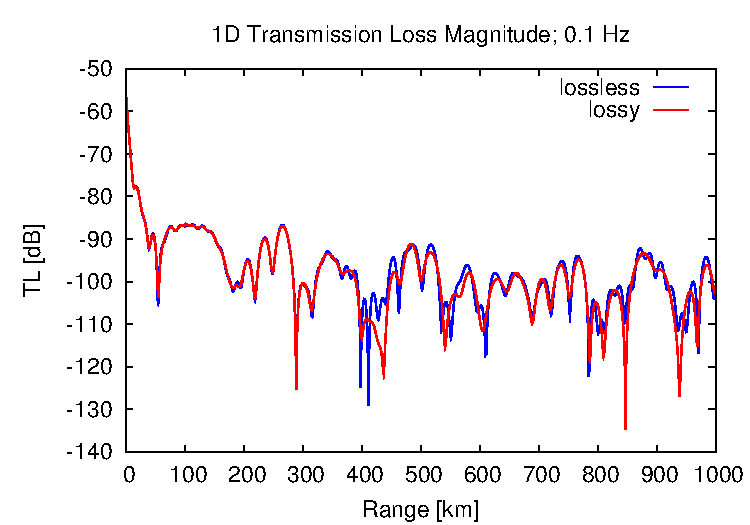
\includegraphics[scale=0.60]{figs/rdmodess_ex1_1d}
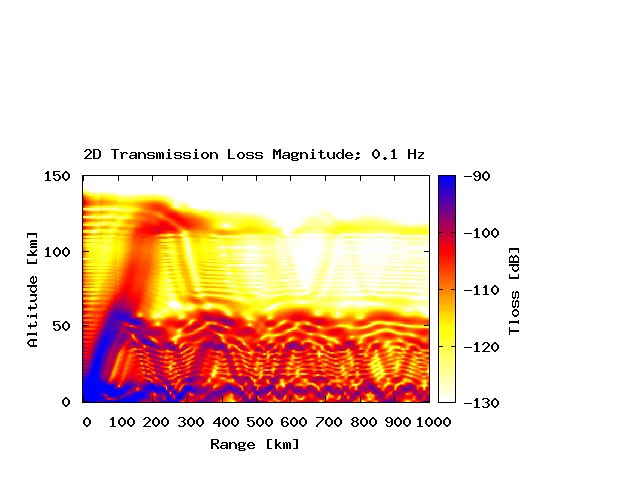
\includegraphics[scale=0.45,trim = 20 20 110 140,clip]{figs/rdmodess_ex1_2d.png}
\end{center}
\caption{1D transmission loss magnitude at 0.1 Hz obtained with {\bf ModessRD1WCM} for eastward ground-to-ground propagation in the range dependent profiles provided in the directory {\tt profiles}. Shown are the 1D lossless transmission loss magnitude and lossy transmission loss magnitude and the 2D lossy transmission loss magnitude.}
\label{fig: rdmodess ex1}
\end{figure}

The following example illustrates the functionality and inputs of ModessRD1WCM using a user-provided G2S {\tt .env} file. 
\begin{verbatim}
    ../bin/ModessRD1WCM --g2senvfile g2sgcp2011012606L.jordan.env \
           --atmosfileorder zuvwtdp --skiplines 1 --azimuth 90 --freq 0.1 \
           --use_profile_ranges_km 50_100_150_200_250 --write_2D_TLoss
\end{verbatim}
The resulting data files are plotted in Figure \ref{fig: rdmodess ex2}. 

\begin{figure}[h]
\begin{center}
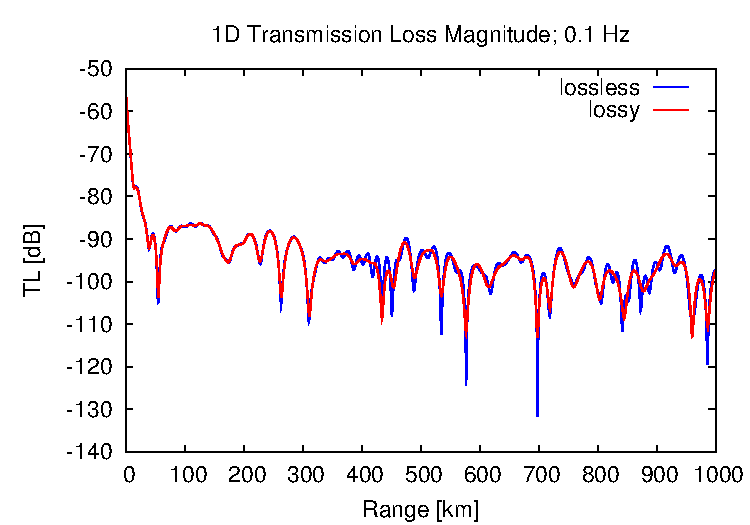
\includegraphics[scale=0.60]{figs/rdmodess_ex2_1d}
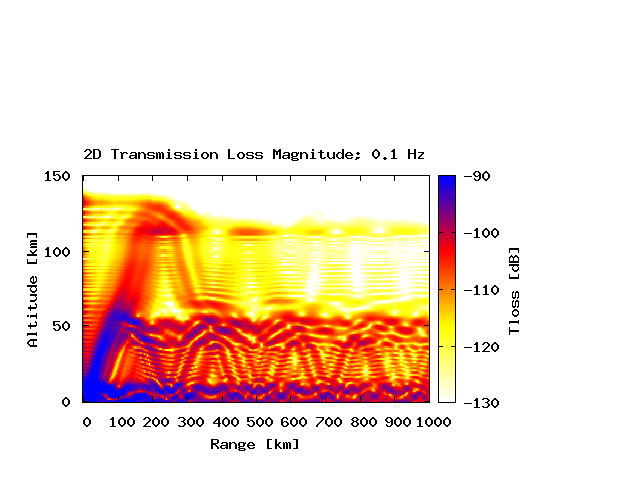
\includegraphics[scale=0.45,trim = 20 20 110 140,clip]{figs/rdmodess_ex2_2d.png}
\end{center}
\caption{1D transmission loss magnitude at 0.1 Hz obtained with {\bf ModessRD1WCM} for eastward ground-to-ground propagation in the range dependent profiles provided by a G2S {\tt .env} binary file. Shown are the 1D lossless transmission loss magnitude and lossy transmission loss magnitude and the 2D lossy transmission loss magnitude.}
\label{fig: rdmodess ex2}
\end{figure}